\chapter{Environnement du travail}
\section{Introduction}
\paragraph{}
Certes, le succées ou l'échec d'un projet informatique dépend du choix des technologies utilisées.
Ce choix dérive essentiellement des objectifs à atteindre et des contraintes d'accompagnement qui doivent être prisent en considération.
\subparagraph{}
Dans cette partie, je vais présenter les différentes technologies envisagées par les architectes de Stample 
et relatives au la développement du Backend (partie sur la quel j'ai travaillé) et le FrontEnd.
Vous trouverez plus de détails sur l'environnement du travail sur ma page\footnote{http://ideas2d.com/moncef/home.php} web.
\section{Working tools}
\subsection{Environnement de Développement}
\begin{itemize}
\item PlayFramework\footnote{http://www.playframework.com/} 2.1.0 : Un Framework open source facilite la creation des APIs web en Scala, Java. Avec Play. Il suffit de recharger la page web pour voir les modiffications de la classe Scala.
\item JDK 7 : Contient les bibliothèques JAVA de base, les outils de compilation et se charge à la transfert du bytecode destiné à la JVM. 
\item Maven3 : Un outil logiciel libre pour la gestion et l'automatisation de production des projets logiciels Java permet la synchronisation des projets indépendants.
\item OS X 10.8.4
\item SBT\footnote{http://www.scala-sbt.org/} 0.12.4 : "simple build tool" Un support pour compiler le code Scala.
\item ElasticSearch\footnote{http://www.elasticsearch.org/} 19.4.0 :  Un moteur de recherche libre vise à offrir des fonctionnalités avancées de recherche à n'import quelle API.
\item MongoDB\footnote{http://www.mongodb.org/} 2.2.x : Un système de gestion de base de données orientée documents(NoSQL). Il permet de manipuler des objets structurés au format BSON (JSON binaire), sans schéma prédéterminé.
\end{itemize}
\subsection{Langages de Programmation}
\begin{itemize}
\item BackEnd : SCALA , JAVA, JSON
\item FrontEnd : HTML5, JavaScript, Jquery, CSS3, JSON, Ajax. 
\end{itemize}
\subsection{Plugins}
\begin{itemize}
\item BackEnd : SecureSocial, Salat, 
\item FrontEnd : Backbonejs 
\end{itemize}
\textbf{SecureSocial} est un plugin permettant d'ajouter une interface utilisateur d'authentification pour votre application qui fonctionne avec des services basés sur OAuth1, OAuth2 et OpenID.
\subsection{Outils de développement}
\begin{itemize}
\item IDE : ItelliJ IDEA 12.1.14 Community Edition;
\item Base de données : Mongodb NoSQL data base;
\item outils de compilation automatique : sbt.
\end{itemize}
\section{Aspects techniques de Stample}
\subsection{Architecture}
\begin{figure}[H]
        \centering
                \centering
                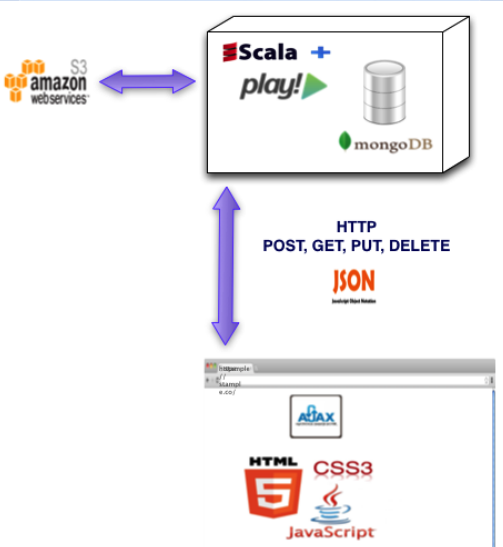
\includegraphics[width=10cm,height=8cm]{architectureStample.png}
                \caption{Architecture de la plateforme}
                \label{fig:Architecture de la plateforme}
       
\end{figure}
\textit{Commentaires : }
La figure 2.1 présente une vu globale sur l'architecture de la plateforme sous forme de trois blocs. On utilise les services web de amazon S3\footnote{http://aws.amazon.com/fr/s3/} pour stocker et extraire des données.
Le deuxième bloc représente le Backend former par "Scala + PlayFramework + Java + MongoDB", on renvoie les données sous forme de JSON au Frontend, les communications sont éffectuées via des requêtes HTTP.
Le troisième bloc présente le Frontend avec tous les outils informatiques de degin "CSS3 + JavaScript + HTML5". Vous aurez plus de détailles sur le Backend par suite. 
\subsection{Description de l'architecture Backend}
\paragraph{}
Les requêtes HTTP sont faites en JSON.
Le JSON est désérialisé dans des objets métiers 
(Scala case class) pour être manipulés au sein de l'application.
\subsubsection{Communication entre la base et l'API}
\paragraph{}
On utilise le driver Casbah\footnote{http://api.mongodb.org/scala/casbah/2.0/tutorial.html} MongoDB en Scala et une librairie "Salat" qui permet une bonne intégration de Casbah dans l'application.
Salat permet de sérialiser les objets métiers (case class) en BSON \footnote{http://bsonspec.org/}, cette libairie propose un DAO (Data Access Object) générique et un model compagnon qui expose les méthodes basique des requêtes Mongo (find(), findById(), search(), ect...)
\subsubsection{Communication entre L'API et ElasticSearch}
\paragraph{}
L’idée d’ElasticSearch est d’offrir une solution de recherche à usage général, qui peut évoluer d’une seule machine à plusieurs centaines.  
L'indexation dans la base se fait manuellement après l'insertion ou la mise à jour d'un document MongoDB dans la base de données.
L'échec d'indexation est non bloquant car il est ratrappé par un traitement spécifique d'exception.
\subparagraph{}
ElasticSearch prend en entrée du JSON cela implique qu'il fontionne particuliérement bien avec Mongo.
De plus, on utilise salat aussi pour produire le JSON d'un objet métier (case class).
Donc nous avons le même document dans MongoDB et ElasticSearch. Cela permet de rendre un document similaire à Backbone pour la recherche.
On utlise un client JAVA pour ElasticSearch.
\subsubsection{SBT}
\paragraph{}
Le "build" est réalisé par SBT, il faudrait mettre en place un outil d'intégration "Jenkins"\footnote{http://fr.wikipedia.org/wiki/Jenkins\_(informatique)} qui fera tourner les tests unitaires et embarqués à chaque "push" d'une branche git pour réparer les regressions et que nous en soyons alertés.
\subsubsection{Les collections MongoDB}
\paragraph{}
Stample structure les données sous forme de différentes collections.
Elles sont toutes identifiées par un ObjectId, elles regroupent toutes les informations nécessaire sur les utilisateurs (Compte utilisateurs, Stamples, ect...).
\newpage
\subsection{Configuration de départ}
\subsubsection{Description de la configuration}
\paragraph{}
Le projet contient de quatre répertoires séparés : \textit{fixturedatabase} contenant les fichiers JSON et leurs sérialisation binaire encodé BSON, \textit{restore} inclu le build de l'application et les plugins, \textit{stample-search} contenant les classes java et la configuration nécessaire pour le lancement du projet et \textit{stample-web} ce dernier contient les diffirents packages du code Front/back End.
\paragraph{}
Afin de participer au projet, j'ai installé les outils cité précédemment dans un premier temps. Ensuite, j'ai configuré ma machine avec les paths nécessaires pour lancer sbt, play, mongo et elasticSearch. Puis, j'ai lancé le mvn dans le répertoire stample-search. Enfin il est indisponsable de lancer play ou sbt et de générer les fichier idea, eclipse ou autre dans stample-web selon l'IDE envisagé.    
Le README.md du projet écrit avec le langage de balisages légers Markdown\footnote{http://fr.wikipedia.org/wiki/Markdown} contient les détails nécessaires pour la configuration du projet.
\subsection{Gestion du travaille en groupe}
\paragraph{}
Les régles du travaille en groupe sur le projet Git :
\begin{enumerate}
\item NE PAS travailler directement sur la branche master. Ce n'est que pour la production.
\item La branche de développement principale est "preProd". A partir de cette branche on commence une nouvelle branche. 
\item Lors du développement sur une branche, merger régulièrement preProd en elle, pour s'assurer d'être à jour avec le travail des autres développeurs.
\item Lorsque la branche est stable et a été testé par le chef de projet, il va tester, merger dans preProd, on peut supprimer le projet.
\item Utiliser toujours camelCase pour nommer les branches et des noms intelligents!
\item Ajouter des explications intelligentes lors de chaque commit.
\end{enumerate}
\section{Conclusion du chapitre 2}
\paragraph{}
Dans ce chapitre introductif, j'ai détaillé les outils qu'on utilise. Ensuite, j'ai présenté l'architécture globale de la plateforme et les diffirentes interractions. Le prochain chapitre présente une idée générale sur le langage de programmation "Scala" du Backend Stample. 
